% Options for packages loaded elsewhere
\PassOptionsToPackage{unicode}{hyperref}
\PassOptionsToPackage{hyphens}{url}
%
\documentclass[
]{article}
\usepackage{amsmath,amssymb}
\usepackage{lmodern}
\usepackage{iftex}
\ifPDFTeX
  \usepackage[T1]{fontenc}
  \usepackage[utf8]{inputenc}
  \usepackage{textcomp} % provide euro and other symbols
\else % if luatex or xetex
  \usepackage{unicode-math}
  \defaultfontfeatures{Scale=MatchLowercase}
  \defaultfontfeatures[\rmfamily]{Ligatures=TeX,Scale=1}
\fi
% Use upquote if available, for straight quotes in verbatim environments
\IfFileExists{upquote.sty}{\usepackage{upquote}}{}
\IfFileExists{microtype.sty}{% use microtype if available
  \usepackage[]{microtype}
  \UseMicrotypeSet[protrusion]{basicmath} % disable protrusion for tt fonts
}{}
\makeatletter
\@ifundefined{KOMAClassName}{% if non-KOMA class
  \IfFileExists{parskip.sty}{%
    \usepackage{parskip}
  }{% else
    \setlength{\parindent}{0pt}
    \setlength{\parskip}{6pt plus 2pt minus 1pt}}
}{% if KOMA class
  \KOMAoptions{parskip=half}}
\makeatother
\usepackage{xcolor}
\IfFileExists{xurl.sty}{\usepackage{xurl}}{} % add URL line breaks if available
\IfFileExists{bookmark.sty}{\usepackage{bookmark}}{\usepackage{hyperref}}
\hypersetup{
  hidelinks,
  pdfcreator={LaTeX via pandoc}}
\urlstyle{same} % disable monospaced font for URLs
\usepackage{graphicx}
\makeatletter
\def\maxwidth{\ifdim\Gin@nat@width>\linewidth\linewidth\else\Gin@nat@width\fi}
\def\maxheight{\ifdim\Gin@nat@height>\textheight\textheight\else\Gin@nat@height\fi}
\makeatother
% Scale images if necessary, so that they will not overflow the page
% margins by default, and it is still possible to overwrite the defaults
% using explicit options in \includegraphics[width, height, ...]{}
\setkeys{Gin}{width=\maxwidth,height=\maxheight,keepaspectratio}
% Set default figure placement to htbp
\makeatletter
\def\fps@figure{htbp}
\makeatother
\setlength{\emergencystretch}{3em} % prevent overfull lines
\providecommand{\tightlist}{%
  \setlength{\itemsep}{0pt}\setlength{\parskip}{0pt}}
\setcounter{secnumdepth}{-\maxdimen} % remove section numbering
\ifLuaTeX
  \usepackage{selnolig}  % disable illegal ligatures
\fi

\author{}
\date{}

\begin{document}

\hypertarget{header-n49}{%
\section{\texorpdfstring{\emph{\underline{Bash
Learning}}}{Bash Learning}}\label{header-n49}}

\hypertarget{header-n42}{%
\subsection{\texorpdfstring{\emph{一. Introduction to LINUX
Systems}}{一. Introduction to LINUX Systems}}\label{header-n42}}

\hypertarget{header-n56}{%
\subsubsection{1.1. The history of LINUX and its
versions}\label{header-n56}}

\begin{quote}
The LINUX system was developed in 1991 by a Finnish university student,
Linus, and a succession of enthusiasts.
\end{quote}

\begin{quote}
LIUNX distributions: the redhat series (redhat, centOS) and the debian
series (debian, ubuntu). Both distributions use the LINUX kernel, so the
basic operations are the same, the main difference is that the software
is installed differently.
\end{quote}

\hypertarget{header-n48}{%
\subsubsection{1.2. Features as open source software}\label{header-n48}}

\begin{quote}
Free, accessible software source code is more secure, distributable and
improved.
\end{quote}

\hypertarget{header-n13}{%
\subsection{\texorpdfstring{\emph{二. Linux common
commands}}{二. Linux common commands}}\label{header-n13}}

\hypertarget{header-n68}{%
\subsubsection{1. Directory processing commands}\label{header-n68}}

\begin{verbatim}
# list

ls  # /-a /-l /-d
\end{verbatim}

\begin{verbatim}
# make directories

mkdir # /-p
\end{verbatim}

\begin{verbatim}
# change directory

cd # /.. /- /~
\end{verbatim}

\begin{verbatim}
# print working directory

pwd 
\end{verbatim}

\begin{verbatim}
# remove empoty directory

rmdir
\end{verbatim}

\begin{verbatim}
# copy

cp # /-r /-p
\end{verbatim}

\begin{verbatim}
# move

mv 
\end{verbatim}

\begin{verbatim}
# remove

rm # /-rf /-i
\end{verbatim}

\hypertarget{header-n88}{%
\subsubsection{2. Document processing commands}\label{header-n88}}

\begin{verbatim}
touch
\end{verbatim}

\begin{verbatim}
cat # /-n

$ cat -n /etc/services
\end{verbatim}

\begin{verbatim}
more # /q /Enter /space

$ more /etc/services
\end{verbatim}

\begin{verbatim}
less # / :/ser (find the specified character,press n to find the next one)

$ less /etc/services
\end{verbatim}

\begin{verbatim}
head # /-n

$ head -n 20 /etc/services
\end{verbatim}

\begin{verbatim}
tail # /-n

$ tail -n 20 /etc/services
\end{verbatim}

\hypertarget{header-n9}{%
\subsubsection{3. Permission management commands}\label{header-n9}}

\begin{verbatim}
# change file mode bits

chmod # / [{ugo} {+-=} {rwx}] [document/directory] / [mode=421] [document/directory]

# r----4, w-----2, x----1

$ chmod g+w testfile

$ chmod 777 testfile

$ chmod -R 777 testfile # recursive modification
\end{verbatim}

\hypertarget{header-n8}{%
\subsubsection{4. Search commands}\label{header-n8}}

\begin{verbatim}
# search the directory where the command is located

which 

$ which ls
\end{verbatim}

\begin{verbatim}
# search within document

grep  # /-i /-v /-n

$ cat sonnet104.txt |grep -n -i -v "three"
\end{verbatim}

\hypertarget{header-n6}{%
\subsubsection{5. Help commands}\label{header-n6}}

\begin{verbatim}
# manual

man 

$ man ls
\end{verbatim}

\begin{verbatim}
help

$ ls --help
\end{verbatim}

\begin{verbatim}
whatis

$ whatis ls
\end{verbatim}

\hypertarget{header-n2}{%
\subsubsection{6. Compression and decompression
commands}\label{header-n2}}

\begin{verbatim}
# GUN zip

gzip  

$ gzip testfile



# GUN unzip

gunzip

$ gunzip testfile
\end{verbatim}

\begin{quote}
gzip and gunzip do not retain the original file after compression and
decompression
\end{quote}

\begin{verbatim}
tar

$ tar -zcvf sonnet104.tar.gz sonnet104.txt

$ tar -zxvf sonnet104.tar.gz
\end{verbatim}

\begin{verbatim}
zip  # /-r (compressed directory)

$ zip sonnet104.zip sonnet104.txt



unzip

$ unzip sonnet104.zip
\end{verbatim}

\begin{quote}
zip and unzip do not retain the original file after compression and
decompression
\end{quote}

\begin{verbatim}
bzip2 # /-k ( retain the original file)

$ bzip2 sonnet104.txt



bunzip2

$ bunzip2 -k sonnet104.txt.bz2
\end{verbatim}

\begin{quote}
bzip2 is an upgraded version of gzip with a very impressive compression
ratio
\end{quote}

\hypertarget{header-n132}{%
\subsection{\texorpdfstring{\emph{三. Text editor
vim}}{三. Text editor vim}}\label{header-n132}}

\begin{quote}
vim is a powerful full-screen text editor that creates, edits and
displays text files
\end{quote}

\begin{figure}
\centering
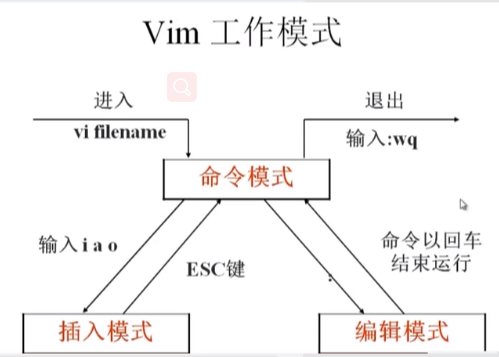
\includegraphics{C:/Users/228/Desktop/vim.png}
\caption{}
\end{figure}

\hypertarget{header-n138}{%
\subsubsection{1. Insert commands}\label{header-n138}}

\begin{verbatim}
a  # Insert after the character where the cursor is located

A  # Insert at the end of the line where the cursor is located

i  # Insert before the character where the cursor is located

I  # Insert at the beginning of the line where the cursor is located

o  # Insert a new line under the cursor

O  # Insert a new line on the cursor
\end{verbatim}

\hypertarget{header-n142}{%
\subsubsection{2. Locate commands}\label{header-n142}}

\begin{verbatim}
:set number     # Set the line number

:set nonumber   # Cancel line number

gg              # Go to first line

G               # Go to the last line

:n              # Go to nth row

$               # Move to end of line

0               # Move to beginning of line
\end{verbatim}

\hypertarget{header-n144}{%
\subsubsection{3. Delete, copy, cut and paste
commands}\label{header-n144}}

\begin{verbatim}
dd         # Delete the line where the cursor is

:n1,n2d    # Delete a specified range of rows



yy         # Copy the line where the cursor is

nyy        # Copy n lines below the cursor line



dd         # Cut the line where the cursor is

ndd        # Cut n lines below the line where the cursor is located



p/P        # Paste under or over the line where the cursor is located
\end{verbatim}

\hypertarget{header-n146}{%
\subsubsection{4. Replace command}\label{header-n146}}

\begin{verbatim}
:%s/old/new/g       # Replace the specified string with the full text



:n1,n2s/old/new/g   # Replace the specified string within a certain range
\end{verbatim}

\hypertarget{header-n150}{%
\subsection{\texorpdfstring{\emph{四.
Shell}}{四. Shell}}\label{header-n150}}

\hypertarget{header-n194}{%
\subsubsection{1. Overview of the shell}\label{header-n194}}

\begin{figure}
\centering
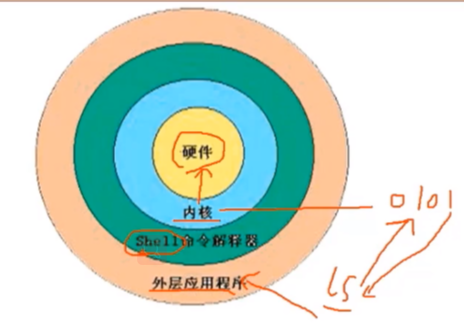
\includegraphics{C:/Users/228/Desktop/shell.png}
\caption{}
\end{figure}

\begin{quote}
The shell is a command line interpreter that provides an interface
system level program for the user to send requests to the Linux kernel
in order to run programs. The user can use the shell to start, hang,
stop, and write a number of programs.
\end{quote}

\begin{quote}
The shell is also a powerful programming language that is easy to write,
debug and very flexible. shell is an interpreted scripting language in
which Linux system commands can be invoked directly.
\end{quote}

\hypertarget{header-n158}{%
\subsubsection{2. Execution of shell scripts}\label{header-n158}}

\hypertarget{header-n276}{%
\subparagraph{2.1. The echo output command}\label{header-n276}}

\begin{verbatim}
echo  # /-e  # Support for backslash-controlled character conversion



$ echo -e \

> 'hello,

>  world!'
\end{verbatim}

\hypertarget{header-n259}{%
\subparagraph{2.2. The first script}\label{header-n259}}

\begin{verbatim}
$ vim hello.sh

#!/bin/bash

#The first script



echo "Hello, world!"
\end{verbatim}

\begin{quote}
Before the script can be executed, it needs to be given execute
permission
\end{quote}

\begin{verbatim}
$ chmod 755 hello.sh

$ ./hello.sh



# Execution is possible without granting execution rights

$ bash hello.sh
\end{verbatim}

\hypertarget{header-n288}{%
\subparagraph{2.3. Output redirection}\label{header-n288}}

\begin{verbatim}
0  # Standard input

1  # Standard output

2  # Standard error output



command > document   #Outputs the correct output to the specified file as an overwrite

command >> document  #Output the correct output to the specified file as an append

error command 2> document

error command 2>> document



command > document 2>&1  #Save both correct and incorrect output to the same file as an overwrite

command >> document 2>&1

command >> document1 2>>document2 #Append the correct output to file 1 and the incorrect output to file 2



# Commonly used example

$ nohup ./hello.sh >run.log 2>&1 &
\end{verbatim}

\hypertarget{header-n298}{%
\subparagraph{2.4. Multi-command sequential execution and pipeline
characters}\label{header-n298}}

\begin{verbatim}
;     command1; command2  #Sequential execution, no logical relationship

&&    command1 && command2 #Logical and, when command 1 is executed correctly, command 2 will be executed

||   command1 || command2  #Logical or, when command 1 is not executed correctly, command 2 will be executed

|    command1 |command2   #Pipeline character with the correct output of command 1 as the operation of command 2



$ ls && echo "yes" || echo "no"



$ cat sonnet104.txt |tr -cs A-Za-z "\n" |sort |uniq -c |sort -n -k 1,1 |awk '$1>2 {print $2}'
\end{verbatim}

\hypertarget{header-n296}{%
\subparagraph{2.5. wildcard character}\label{header-n296}}

\begin{verbatim}
?     #Match a character

*     #Match 0 or any number of arbitrary characters

[]    #Match any of the characters in the brackets  [abc]

[-]   #Match any of the characters in the brackets  [a-z]

[^]   #Logical non, matches characters not in brackets [^0-9]



$ touch abc abcd 012 0abc

$ ls

$ ls ?abc

$ ls [^0-9]*

$ ls [0-9]*
\end{verbatim}

\hypertarget{header-n302}{%
\subparagraph{2.6. Other special symbols}\label{header-n302}}

\begin{verbatim}
``    #Anti-quote. The content enclosed in backquotes is a system command, and serves the same purpose as $().

""    #Double inverted commas. None of the special symbols in double quotes have a special meaning, but $ and \ have a special meaning

''  #Single inverted commas. All special symbols in single inverted commas have no special meaning.

$()   #Referencing system commands

$    #Calling variables

\    #Escape character



$ name=lsw

$ echo '$name'

$ echo "$name"

$ echo '$(date)'

$ echo "$(date)"
\end{verbatim}

\hypertarget{header-n270}{%
\subsubsection{3. Variables in Bash}\label{header-n270}}

\begin{quote}
Variables are bits of computer memory in which the values stored can be
changed. Each variable has a name, so it is easy to refer to it. The use
of variables allows useful information or temporary information to be
stored.
\end{quote}

\hypertarget{header-n275}{%
\subparagraph{3.1. User-defined variables}\label{header-n275}}

\begin{quote}
Effective only in the current shell
\end{quote}

\begin{verbatim}
# Defining variable

$ name="Shengwei Li"



# Defining variable

$ aa=123

$ aa="$aa"456

$ aa=${aa}789



# Calling variable

$ echo $name



# View variable

$ set



# Delete variable

$ unset name
\end{verbatim}

\hypertarget{header-n311}{%
\subparagraph{3.2. Environment variables}\label{header-n311}}

\begin{quote}
This variable mainly stores data related to the operating environment of
the system
\end{quote}

\begin{quote}
Environment variables can take effect in the current shell and all
sub-shells. If written to a configuration file, it will take effect in
all shells.
\end{quote}

\begin{verbatim}
# Setting environment variable

$ export name="shengwei li"



# Query variable

$ env



# Delete variable

$ unset name
\end{verbatim}

\begin{verbatim}
# Common environment variables - PATH

$ echo $PATH



$ PATH="$PATH":/home/bioinfo/sh
\end{verbatim}

\hypertarget{header-n333}{%
\subparagraph{3.3. Position parameter variables}\label{header-n333}}

\begin{quote}
This variable is mainly used to pass parameters or data into the script
\end{quote}

\begin{verbatim}
$n   #$1-$9 for the first to ninth arguments, ${10}

$*   #Represents all parameters, looking at all parameters as a whole

$@   #Represents all parameters, but treats each parameter differently

$#   #Represents the number of all parameters
\end{verbatim}

\begin{verbatim}
$ vim sum.sh



#!/bin/bash



num1=$1

num2=$2

num3=$3



sum=$(( $num1+$num2+$num3 ))

echo $sum



echo "A total of $# parameters"



echo "The parameters is $@."



echo "The parameter is $*."



$ chmod 755 sum.sh

$ ./sum.sh 1  2 3
\end{verbatim}

\hypertarget{header-n273}{%
\subparagraph{3.5. Predefined variables}\label{header-n273}}

\begin{quote}
This variable is one that is already defined in bash
\end{quote}

\begin{verbatim}
# Receive keyboard input

read  # /-p /-t /-n /-s
\end{verbatim}

\begin{verbatim}
$ vim read.sh



#!/bin/bash



read -t 30 -p "Pleace enter your name: " name



echo "Hello, $name."



read -t 30 -s -p "Pleace enter your age: " age



echo -e "\n"

echo "You are $age years old now."



read -t 30 -n 1 -p "Pleace enter your gender:[M/F] " gender

echo -e "\n"

echo "Your gender is $gender"
\end{verbatim}

\hypertarget{header-n203}{%
\subsubsection{4. Shell programming}\label{header-n203}}

\hypertarget{header-n346}{%
\subparagraph{4.1. cut, awk, sed}\label{header-n346}}

\begin{verbatim}
# cut: field extraction command (intercept eligible columns, tab separated by default)

cut  # /-f /-d



$ cut -f 2 student.txt 

$ cut -f 2,3 student.txt 

$ cut -d ":" -f 1,3 /etc/passwd



# Limitations of the cut command

$ df -h |cut -d "" -f 1,3
\end{verbatim}

\begin{verbatim}
# awk command (reads by row, intercepts eligible columns; FS specifies separator)

awk 'pattern1{action1} pattern2{action2}...'  document



## pattern

x>10

x>=10

x<=10

## action

1. Formatted output 

2. flow control statements



$ cat student.txt |awk '$4>80 {print $2}'





## print command (Generally used in the awk command)

$ awk '{print $2 "\t" $3}' student.txt

$ df -h |awk '{print $1 "\t" $3}'



## BEGIN, FS, END 

$ cat student.txt |awk 'BEGIN {print "Transcript \n"} {print $2 "\t" $4}'



$ cat /etc/passwd |grep "/bin/bash" |awk 'BEGIN {FS=":"} {print $1 "\t" $3}'



$ cat student.txt |awk 'END {print "End \n"} {print $2 "\t" $4}'
\end{verbatim}

\begin{verbatim}
# sed command (line operation, which differs from vim in that not only can you modify the contents of a file, but also supports pipe operations, which can modify the result of a command)



# sed is a lightweight stream editor for selecting, replacing, deleting and adding commands to data



sed [option] '[action]' document



## option

-n  # Outputting command-processed data to the screen

-e  # Allows multiple sed commands to be applied to input data

-i  # Save the results of the changes directly to a file



## action

a  # add

c  # row replacement

i  # insert

d  # delete

p  # print

s  # string replacement



$ sed '2p' student.txt 

$ sed -n '2p' student.txt 

$ sed '2,4d' student.txt 

$ sed '2a hello' student.txt 

$ sed '2i hello' student.txt 

$ sed '2c No such person' student.txt 

$ sed '3s/Zhang/ZHANG/g' student.txt 

$ sed -i '3s/Zhang/ZHANG/g' student.txt 

$ cat student.txt 

$ sed -e 's/Li/LI/g; s/si/SI/g' student.txt
\end{verbatim}

\hypertarget{header-n353}{%
\subparagraph{4.2. sort, uniq, wc}\label{header-n353}}

\begin{verbatim}
sort [option] document



## option

-u  # remove duplicate rows

-r  # reverse sorting

-o  # write the results to a file  / sort -r number.txt -o number.txt

-n  # sorting by numeric type

-t  # specify the separator

-k  # sort by the specified field



$ sort /etc/passwd

$ sort -r /etc/passwd

$ sort -t ":" -k 3,3 /etc/passwd

$ sort -n -t ":" -k 3,3 /etc/passwd
\end{verbatim}

\begin{verbatim}
uniq [option] document



## option

-c  # display the number of times the row recurs next to each column

-d  # show only recurring rows



$ cat sonnet104.txt |tr -cs A-Za-z '\n' |sort |uniq -c |sort -n -k 1,1 |awk '$1>2 {print $2}'

$ cat sonnet104.txt |tr -cs A-Za-z '\n'|sort |uniq -c -d
\end{verbatim}

\begin{verbatim}
wc [option] document



## option

-l

-w

-m
\end{verbatim}

\hypertarget{header-n365}{%
\subparagraph{4.3. Process control}\label{header-n365}}

4.3.1 if

\begin{verbatim}
#-----------------------

if [ condition ]

	then

		process

fi



$ if [ $(ps -ef | grep -c "ssh") -gt 1 ]; then echo "true"; fi



#----------------------

if [ condition ]

	then

		process1

	else

		process2

fi





#----------------------

if [ condition ]

	then

		process1

elif [ condition2 ]

	then

		process2

elif [ condition3 ]

	then

		process3

else

	process4

fi





#----------------------

vim used.sh



#!/bin/bash

# counting root partition usage



rate=$(df -h |grep "sda3" |awk '{print $5}' |cut -d "%" -f 1)



echo $rate



if [ $rate -ge 10 ]

	then

		echo "Warning! /dev/sda3 is full.rate= $rate."

fi
\end{verbatim}

4.3.2 case

\begin{verbatim}
case $variable in

	value1)

		process1;;

	value2)

		process2;;

	value3)

		process3;;

esac



#-------------------

vim case.sh



#/bin/bash



# determining user input



read -t 30 -p "Do you want to continue? [Y/N]"  i



case $i in

	Y | y)

		echo "ok, we will continue!";;

	N | n)

		echo "OK, Good By.";;

	*)

		echo "error choice.";;

esac
\end{verbatim}

4.3.3 for

\begin{verbatim}
#-----------

for variable in item1 item2 item3

	do

		process

	done

	

$ for var in item1 item2 ... itemN; do command1; command2… done;



#--------------

for((value;condition;change))

	do

		process

	done



#------------------

vim for1.sh



#!/bin/bash

# Printing time



for time in morning noon afternoon evening

	do

		echo "This time is $time!"

	done



#---------------

vim for2.sh



#/bin/bash



#0+1+2+...+100



s=0



for (( i=1;i<101;i=i+1 )) 

	do

		s=$(( $s+$i ))

	done



echo "The result of 1+2+...+100= $s."
\end{verbatim}

4.3.4 while

\begin{verbatim}
while [ condition ]

	do

		process

	done

	

#----------------------

#!/bin/bash



#0+1+2+...+100



i=1

s=0



while [ $i -le 100 ]

	do

		s=$(( $s+$i ))

		i=$(( $i+1 ))

	done



echo "The result of 1+2+...+100= $s."
\end{verbatim}

4.3.5 until

\begin{verbatim}
# The until loop is the opposite of the while loop in that it loops if the condition does not hold, and terminates once it does.



#----------------------

vim until.sh



#!/bin/bash



#0+1+2+...+100



i=1

s=0



until [ $i -gt 100 ]

	do

		s=$(( $s+$i ))

		i=$(( $i+1 ))

	done



echo "The result of 1+2+...+100= $s."
\end{verbatim}

\end{document}
